\documentclass[10pt,a4paper]{article}
\usepackage[utf8]{inputenc}
\usepackage[english]{babel}
\usepackage[T1]{fontenc}
\usepackage{amsmath}
\usepackage{amsfonts}
\usepackage{amssymb}
\usepackage{subcaption}
\usepackage{makeidx}
\usepackage{graphicx}
\usepackage{fourier}
\usepackage{listings}
\usepackage{color}
\usepackage{hyperref}
\usepackage[left=2cm,right=2cm,top=2cm,bottom=2cm]{geometry}
\author{Tommy Müller, Marcus Dittrich, Vincent Noculak}
\title{Holografie}


\begin{document}

\maketitle
\newpage
\tableofcontents
\newpage


\section{Kohärenzlänge des He-Ne-Lasers}

Mithilfe eines Michelson-Interferometers haben wir durch Aufnahme der Kontrastfunktion, in Abhängigkeit des Weglängenunterschieds der beiden aufgeteilten Laserstrahlen, die Kohärenzlänge des von uns verwendeten He-Ne-Lasers bestimmt. Wir definieren die Kohärenzlänge als den Weglängenunterschied, bei dem der Kohärenzgrad einen Wert von $\frac{1}{e}$ hat. Zum Berechnen des Kohärenzgrades $K$ haben wir die maximale und minimale Intensität, $I_{max}$ und $I_{min}$, des Interferenzmusters der Laserstrahlen für verschiedene Weglängenunterschiede $z$ aufgenommen. Den Weglängenunterschied haben wir mit einem Maßband abgemessen. Den Ablesefehler schätzen wir auf $0,1$cm. Weil der Weglängenunterschied zwei mal der verstellte Abstand des Spiegels ist, beträgt der Fehler $\Delta z = 0,2$cm. Unsere Messdaten können in Tabelle \ref{ko1} und \ref{ko2} gesehen werden. Bei den ersten Messungen haben wir den halbdurchlässigen Spiegel falsch herum eingebaut(Tabelle \ref{ko2}), wodurch wir nicht zur Bestimmung der Kohärenzlänge auswertbare Messergebnisse erhielten. Die Messergebnisse für den richtigen Versuchsaufbau sind in Tabelle \ref{ko1} zu sehen. Zur Bestimmung von $I_{max}$ und $I_{min}$ wurde die Intensität des Interferenzmuster an einem Detektor gegen die Zeit gemessen. Durch aktive Erschütterung des Messaufbaus wurde das Interferenzmuster periodisch kurzzeitig verschoben. Folglich nahm der Detektor mehrfach Minima und Maxima des Interferenzmusters auf. Am Computer konnte ein geeigneter Wert, der möglichst wenig von den meisten aufgenommenen Minima oder Maxima abwich, für das Minimum und Maximum des Musters bestimmt werden. Für den Fehler dieses Wertes wurde durch die Standardabweichung zu den Minima oder Maxima verwendet.

Der Kontrastwert eines Interferenzmuster lässt sich berechnen mit $K = \frac{I_{max} - I_{min}}{I_{max} + I_{min}}$. Durch Gaußsche Fehlerfortpflanzung ergibt sich für den Fehler von K

\begin{equation}
	\Delta K = \sqrt{\left(\frac{2I_{min}}{(I_{max} + I_{min})^2}\right)^2(\Delta I_{max}^2) + \left(\frac{-2I_{max}}{(I_{max} + I_{min})^2}\right)^2(\Delta I_{min}^2)}
\end{equation}

Die berechneten Werte für $K$ und $\Delta K$ unserer Messwerte sind in Tabelle \ref{ko1} und \ref{ko2} angegeben.

In Abbildung \ref{kopl2} sind die Werte des Kohärenzgrades aus Tabelle \ref{ko2} dargestellt. Daran, dass die Messwerte nicht Symmetrisch zum Nullwert der Y-Achse sind, lässt sich folgern, dass das Experiment nicht richtig aufgebaut ist. Bei einem richtig eingebauten halbdurchlässigen Spiegel sollten die Messwerte wegen der Symmetrie, dass es keinen Unterschied macht, welcher der beiden Laserstrahlen den längeren Weg zurücklegt, Symmetrisch zum Nullpunkt der y-Achse sein. Aus diesem Plot lässt sich nicht die Kohärenzlänge des Lasers bestimmt.

Die Darstellung des Kohärenzgrades gegen Weglängenunterschied der Laserstrahlen für den richtigen Versuchsaufbau ist in Abbildung \ref{kopl1} zu sehen. Es sind die Werte aus Tabelle \ref{ko1} dargestellt. Es ist zu erkennen, dass der Kohärenzgrad nicht monoton für größere z abfällt. Nach einem Maximum bei $0$cm Weglängenunterschied folgt ein zweites bei $13$cm. Ein Ursache hierfür könnte sein, dass der He-Ne-Laser kein Einmodenlaser ist. Dadurch strahlt er Licht mehrerer Wellenlängen aus. Dies hat Auswirkungen auf das Interferenzmuster der beiden Lichtstrahlen, denn es kommt zu Schwebungseffekten. Als Folge können mehrere Maxima in der Kohärenzfunktion $K(z)$ vorkommen.

In der Abbildung ist der Wert des Kohärenzgrades eingezeichnet, bei dem wir die Kohärenzlänge definieren. Wir fitten K(z) durch unsere Messpunkte mithilfe einer Gauß-Funktion. Zusätzlich plotten wir zwei Gaußfunktionen, die für unsere Messwerte mit jeweils hinzuaddierten und wegsubtrahierten Fehlern gefittet sind. Mithilfe dieser Funktionen bestimmen wir den Fehler der von uns bestimmten Kohärenzlänge. Dazu vergleichen wir den Wert der Kohärenzlänge unserer Ausgleichskurve und der Fehlerkurven. Die größte Differenz der Kohärenzlängen von Ausgleichs- und Fehlerkurve nehmen wir als Fehler. Mit dieser Vorgehensweise erhalten wir für unsere Messung eine Kohärenzlänge von $(24,5 \pm 0,6)cm$.

Bei der Aufnahme von Hologrammen haben unsere Laserstrahlen einen Weglängenunterschied von weniger als $10cm$, bevor sie im Film interferieren. Die Kohärenzlänge des He-Ne-Lasers reicht deshalb in unserem Experiment zur Aufnahme von Hologrammen aus.



\begin{table}[h!]
	\centering
	\begin{tabular}{|l|l|l|l|l|l|l|}\hline
		$z \pm 0,2$ in cm & $I_{max}$ in V & $\Delta I_{max}$ in V & $I_{min}$ in V & $\Delta I_{min}$ in V & K & $\Delta K$\\\hline
	0,0 & 3,3	& 0,1	& 0,32	& 0,08	& 0,82&		0,05\\
	2,0&	2,89&	0,05&	0,53&	0,06&	0,69 &	0,03\\
	6,0&	3,48&	0,09&	0,32&	0,09&	0,83&	0,05\\
	10,0&	3,30&	0,08&	0,24&	0,13&	0,86&		0,07\\
	13,0&	4,77&	0,05&	0,82&	0,07&	0,71&	0,03\\
	15,0&	4,39&	0,09&	1,06&	0,07&	0,61&	0,03\\
	17,0&	4,59&	0,03&	1,13&	0,09&	0,60&	0,03\\
	19,0&	4,16&	0,04&	1,40&	0,05&	0,50&	0,02\\
	21,0&	3,97&	0,04&	1,68&	0,05&	0,41&	0,02\\
	23,0&	4,14&	0,02&	1,88&	0,04&	0,38&	0,01\\
	25,0&	3,92&	0,03&	1,91&	0,02&	0,34&	0,01\\
		\hline
	\end{tabular}
	\caption{Gemessene Werte für die Intensitäten des Interferenzmusters am Michelson-Interferometers für verschiedene Weglängenunterschiede der Laserstrahlen}
	\label{ko1}
\end{table}

\begin{table}[h!]
	\centering
	\begin{tabular}{|l|l|l|l|l|l|l|}\hline
		$z \pm 0,2$ in cm & $I_{max}$ in V & $\Delta I_{max}$ in V & $I_{min}$ in V & $\Delta I_{min}$ in V & K & $\Delta K$\\\hline
		-14,0&	3,13&	0,04&	1,11&	0,04&	0,48&	0,02\\
		-10,0&	3,19&	0,04&	1,05&	0,04&	0,50&	0,02\\
		-6,0&	3,73&	0,06&	0,61&	0,07&	0,72&	0,03\\
		-2,0&	4,01&	0,12&	0,28&	0,04&	0,87&	0,02\\
		 0,0&	4,06&	0,04&	0,3&	0,04&	0,86&	0,02\\
		 2,0&	4,24&	0,06&	0,17&	0,07&	0,92&	0,04\\
		 4,0&	4,05&	0,05&	0,19&	0,07&	0,91&	0,04\\
		 6,2&	4,03&	0,1&	0,3&	0,07&	0,86&	0,04\\
		 8,0&	4,15&	0,12&	0,18&	0,09&	0,92&	0,04\\
		 8,8&	4,19&	0,07&	0,33&	0,09&	0,85&	0,04\\
		 18,0&	2,79&	0,03&	1,41&	0,03&	0,33&	0,01\\
		
		\hline
	\end{tabular}
	\caption{Gemessene Werte für die Intensitäten des Interferenzmusters am Michelson-Interferometers für verschiedene Weglängenunterschiede der Laserstrahlen bei falsch herum eingebauten halbdurchlässigen Spiegel }
	\label{ko2}
	\end{table}
	
	\begin{figure}[h]
		\centering
		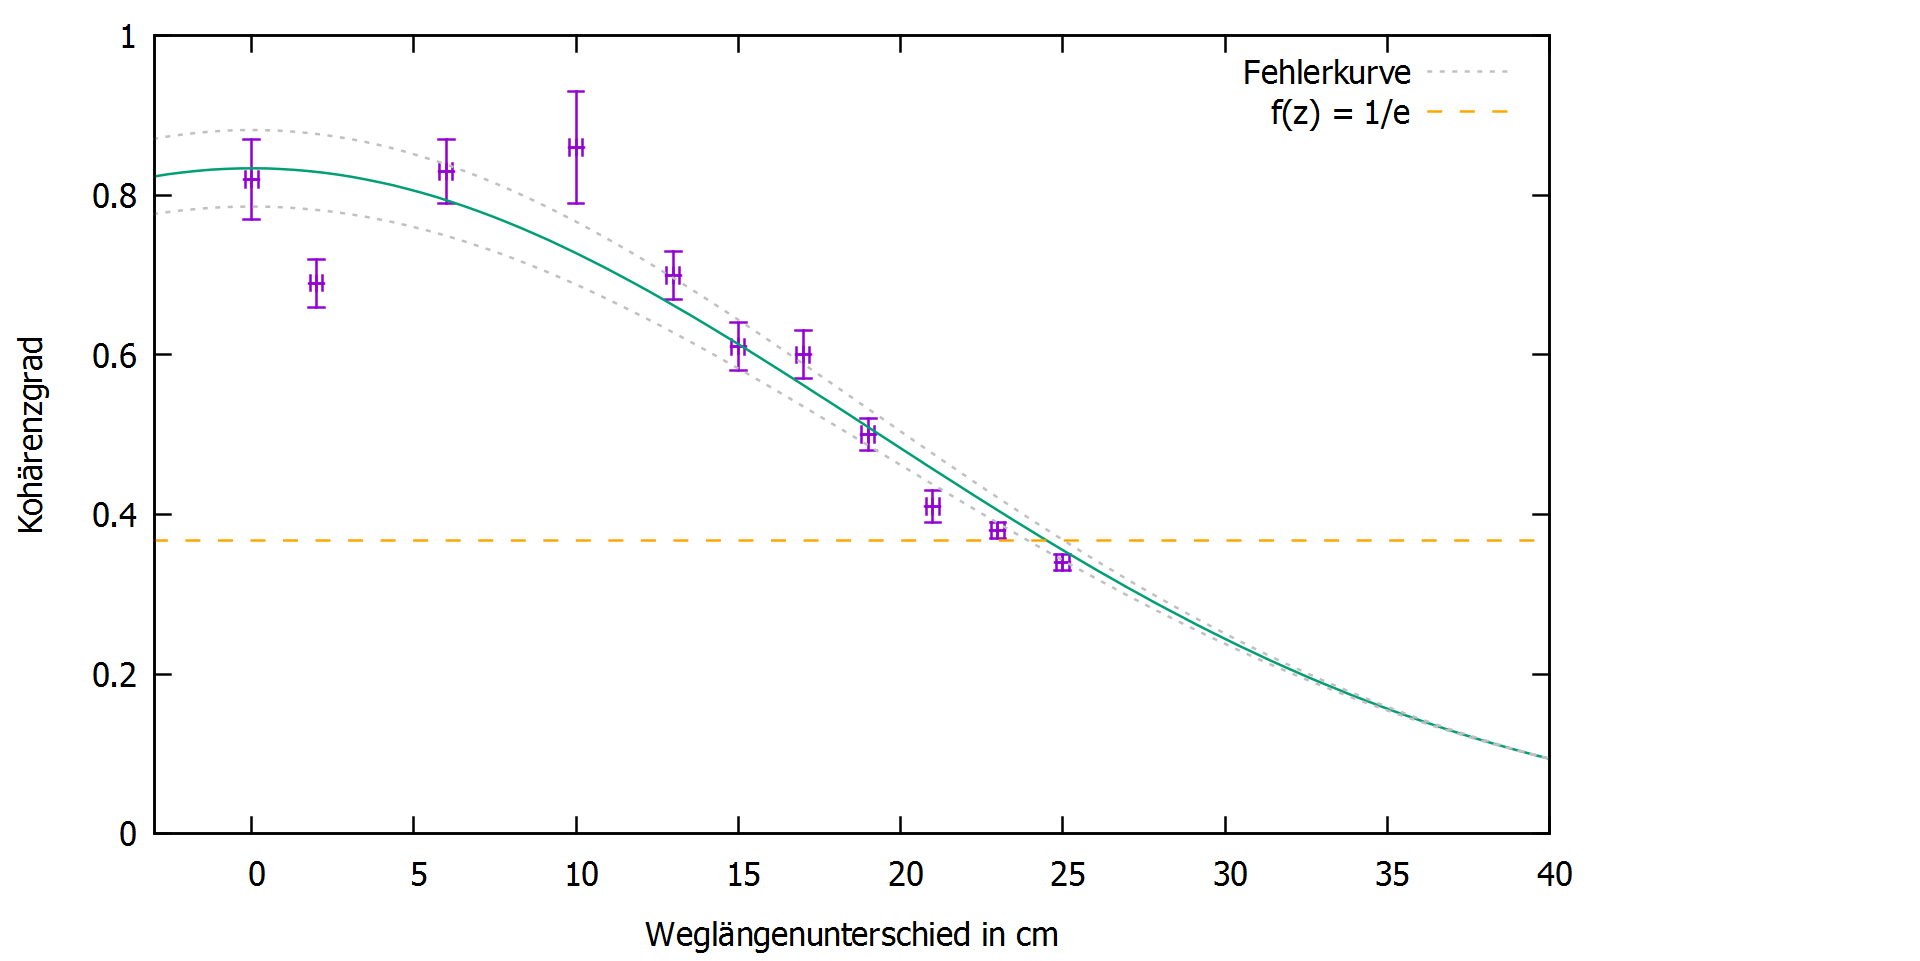
\includegraphics[scale = 0.3]{koplot.png}
		\caption{Kohärenzgrad gegen den Weglängenunterschied der Laserstrahlen im Michelson-Interferometers}
		\label{kopl1}
	\end{figure}
	
		\begin{figure}[h]
			\centering
			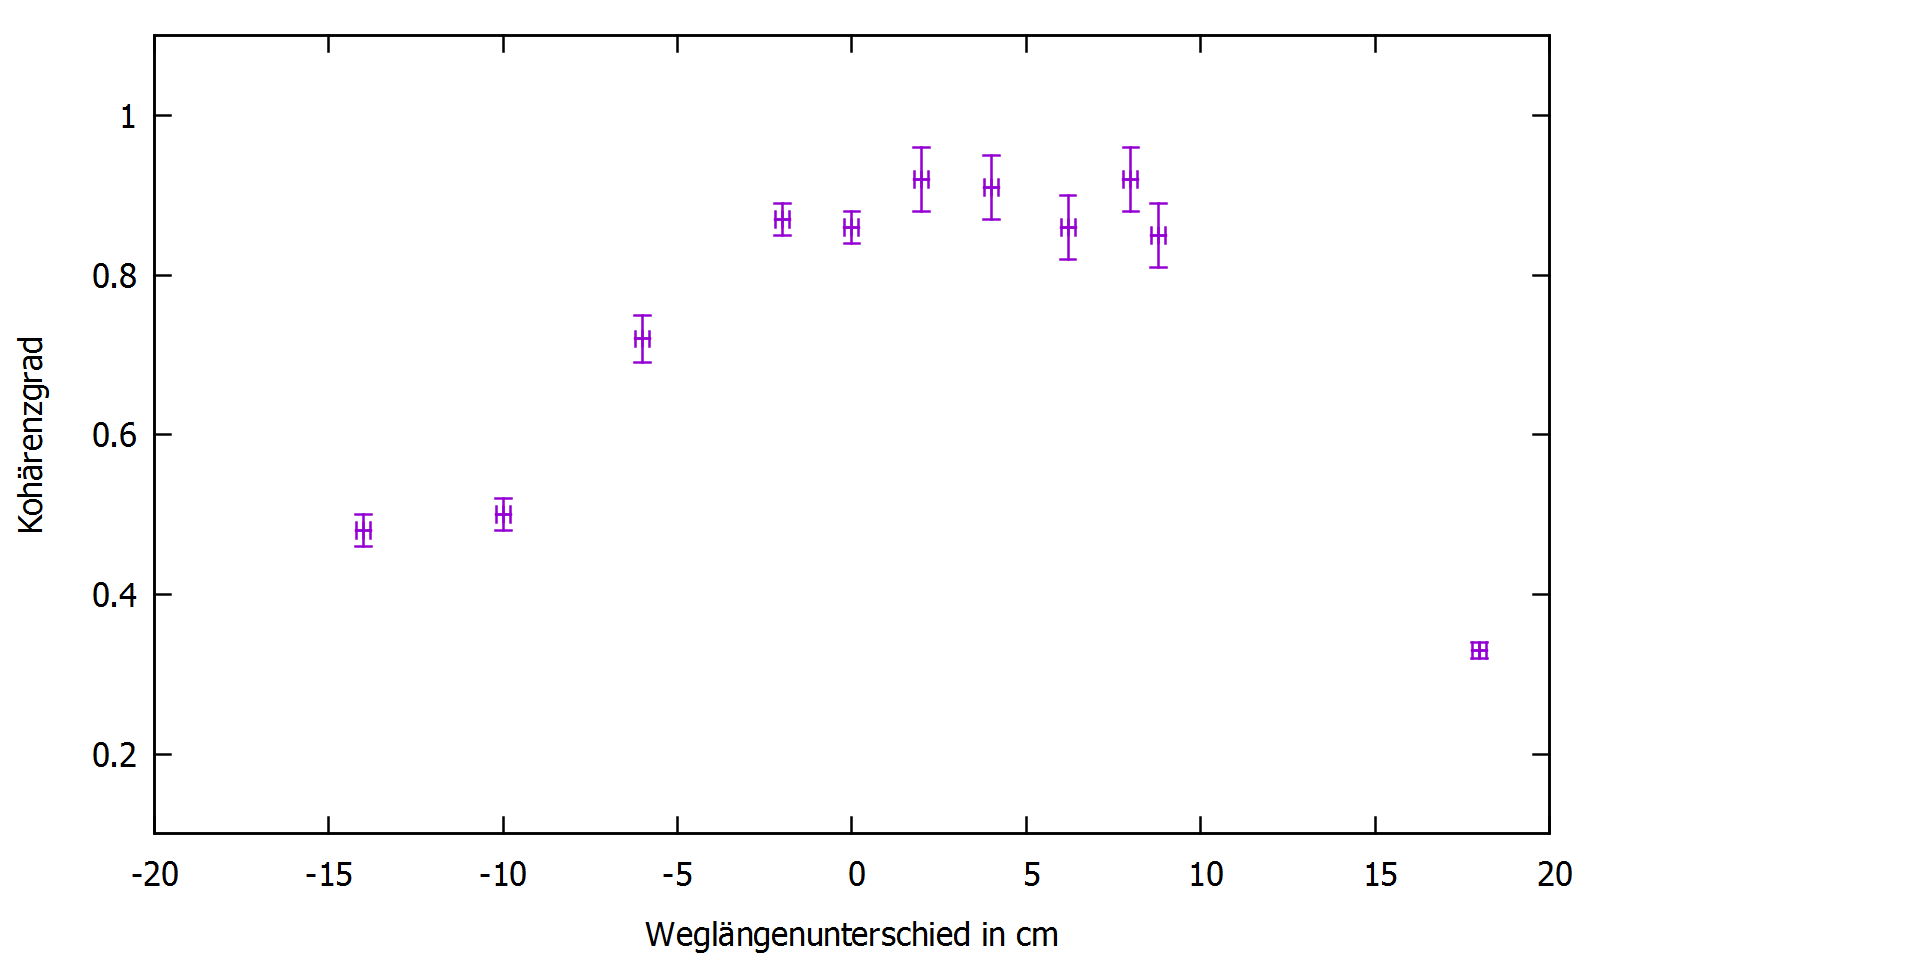
\includegraphics[scale = 0.3]{falsches_koplot.png}
			\caption{Kohärenzgrad gegen den Weglängenunterschied der Laserstrahlen im Michelson-Interferometers für einen falsch herum eingebauten halbdurchlässigen Spiegel}
			\label{kopl2}
		\end{figure}

\subsection{Störungen des Interferenzbildes}

Wir haben die Verschiebung des Interferenzbildes in Abhängigkeit von äußeren Störquellen untersucht. Dazu haben wir die Intensität des Interferenzbildes am festen Ort 45 Sekunden gemessen und währenddessen verschiedene Störungen verursacht. Die Messung kann in Abbildung \ref{stor1} gesehen werden. Während der Messung haben wir neben dem Versuchsaufbau laut geredet und sind umhergelaufen. Zusätzlich haben wir die Tür des Versuchsraums geöffnet und geschlossen und haben kurzzeitig am Untergrund des Versuchsaufbaus gerüttelt. 

Die Störung durch das Rütteln am Untergrund des Versuchaufbaus, kann als Referenz für eine Verschiebung des Interferenzbildes um $\frac{\lambda}{2}$ verwendet werden, da diese Störung sehr intensiv ist. Diese Störung ist in der Abbildung bei $15000ms$ zu sehen. Sie erzeugt eine Spannungsdifferenz von $4V$. Unsere Störungen waren im Vergleich zu den Störungen während der Aufnahme der Hologramme vergleichsweise stark. Über die meiste Zeit der Störungsmessung, von $18000ms$ bis $38000ms$, erzeugen die Störungen eine Spannungsdifferenz im Bereich um $1V$. Das sind $25\%$ der Intensitätsdifferenz von einer Verschiebung um $\frac{\lambda}{2}$. 

Weil wir während der Störungsmessung nahezu durchgehend Störungen erzeugt haben, fällt es schwer die Beruhigungszeit des Aufbaus zu bestimmen. In Abbildung \ref{be1} haben wir zwei Beispiele für eine Beruhigung des Messaufbaus nach einer Störung herausgesucht. Bei \ref{bea} handelt es sich um eine kleine kurzzeitige Störung. Die Störung hat einen Peak bei $11600ms$ und erzeugt eine Spannungsdifferenz von einem Volt. Der Versuchsaufbau benötigt näherungsweise $250ms$ um sich zu beruhigen. In Abb. \ref{beb} kann eine größere Störung, hervorgerufen durch das Rütteln am Untergrund des Versuchsaufbaus gesehen werden. Die Störung ist maximal bei $15000ms$, wo sie eine Spannungsdifferenz von $4V$ erzeugt, und braucht zur Beruhigung bis zur Zeit $17500ms$. Sie hat also eine Beruhigungszeit von $2500ms$. Es fällt auf, dass die Schwankung der Spannung nach $15000$ nicht monoton abnimmt. Dies deutet darauf hin, dass während der Beruhigungszeit der Störung von $15000ms$ eine neue Störung Einfluss auf den Versuchsaufbau nimmt. Dies würde erklären, warum die Beruhigungszeit der Störung aus Abb. \ref{beb} das 10-fache der Beruhigungszeit der Störung aus Abb. \ref{bea} beträgt. 

Aus den beiden Abbildungen lässt sich hauptsächlich erkennen, dass die Beruhigungszeit einer großen Störung länger, als die einer kleinen Störung ist. Zusätzlich lässt sich aus dem Verlauf der Kurven vermuten, dass die Intensität einer Störung während der Beruhigungszeit exponentiell abfällt.

	\begin{figure}[h]
		\centering
		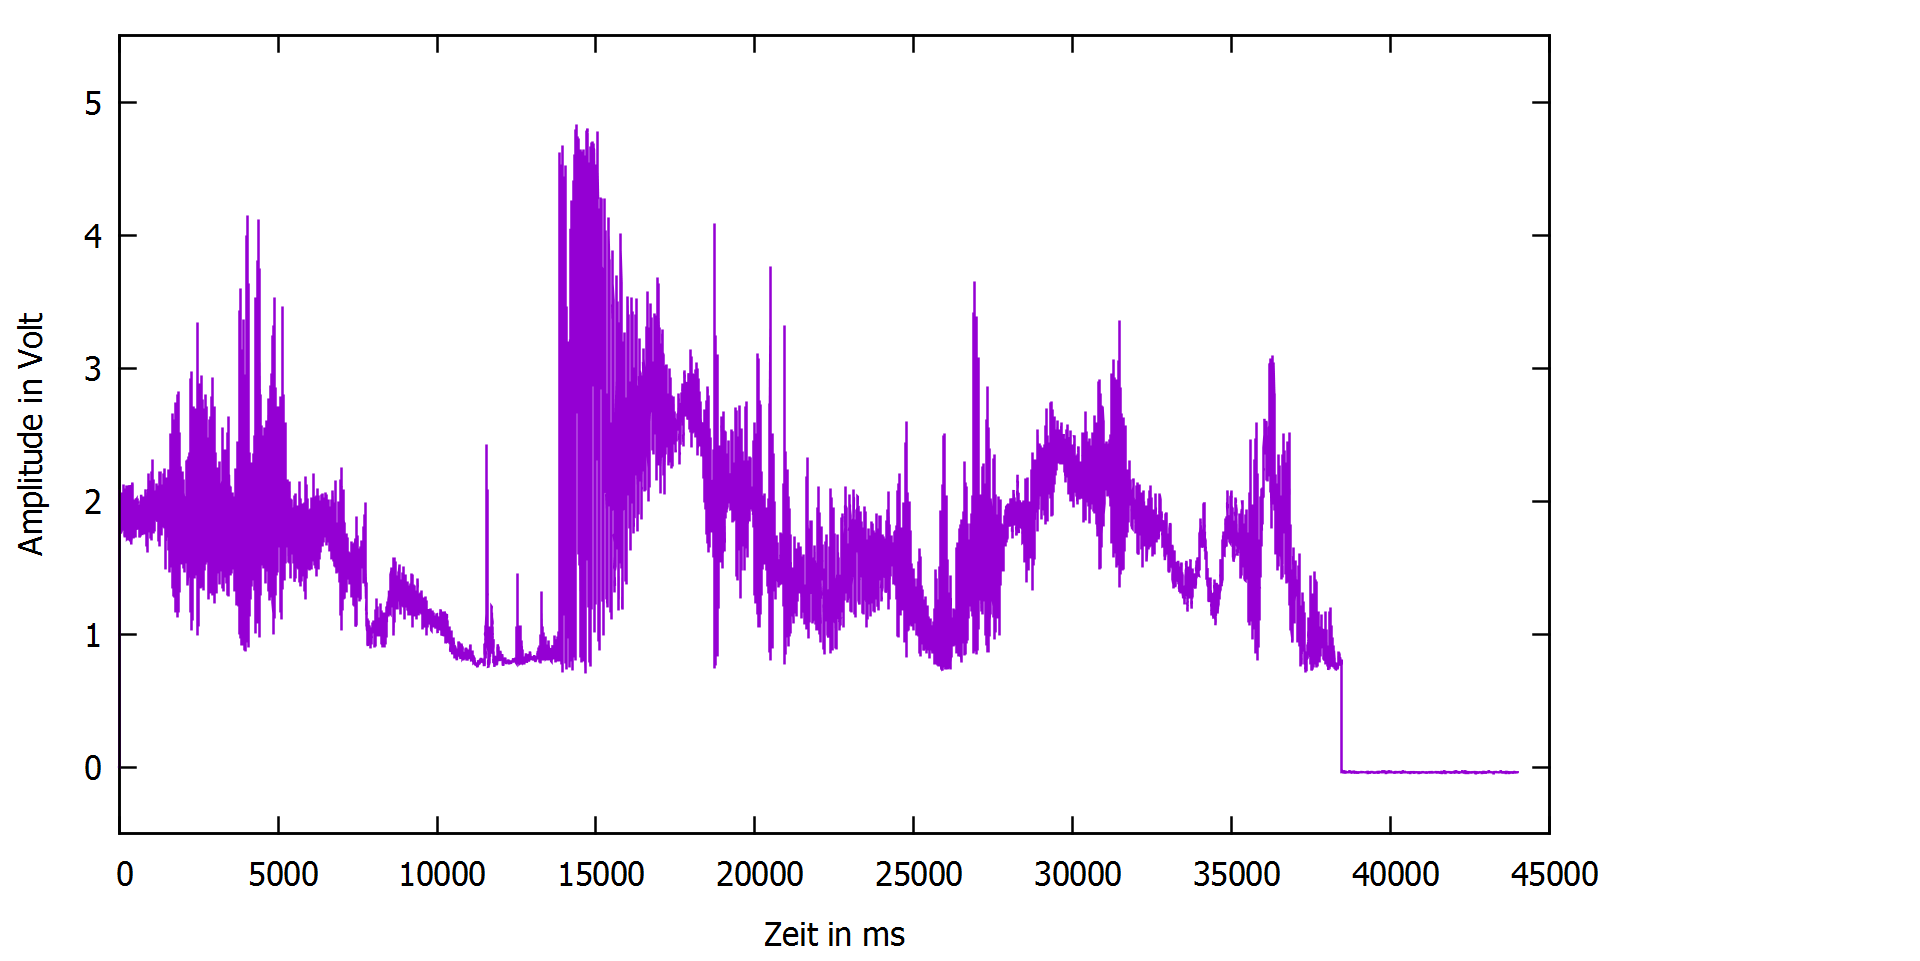
\includegraphics[scale = 0.26]{storung.png}
		\caption{Intensität des Interferenzbildes, aufgetragen gegen die Zeit bei aktiver Erzeugung von Störquellen}
		\label{stor1}
	\end{figure}
	
	\begin{figure}[h]
		\centering
		\begin{subfigure}{0.8\textwidth}
			\centering
			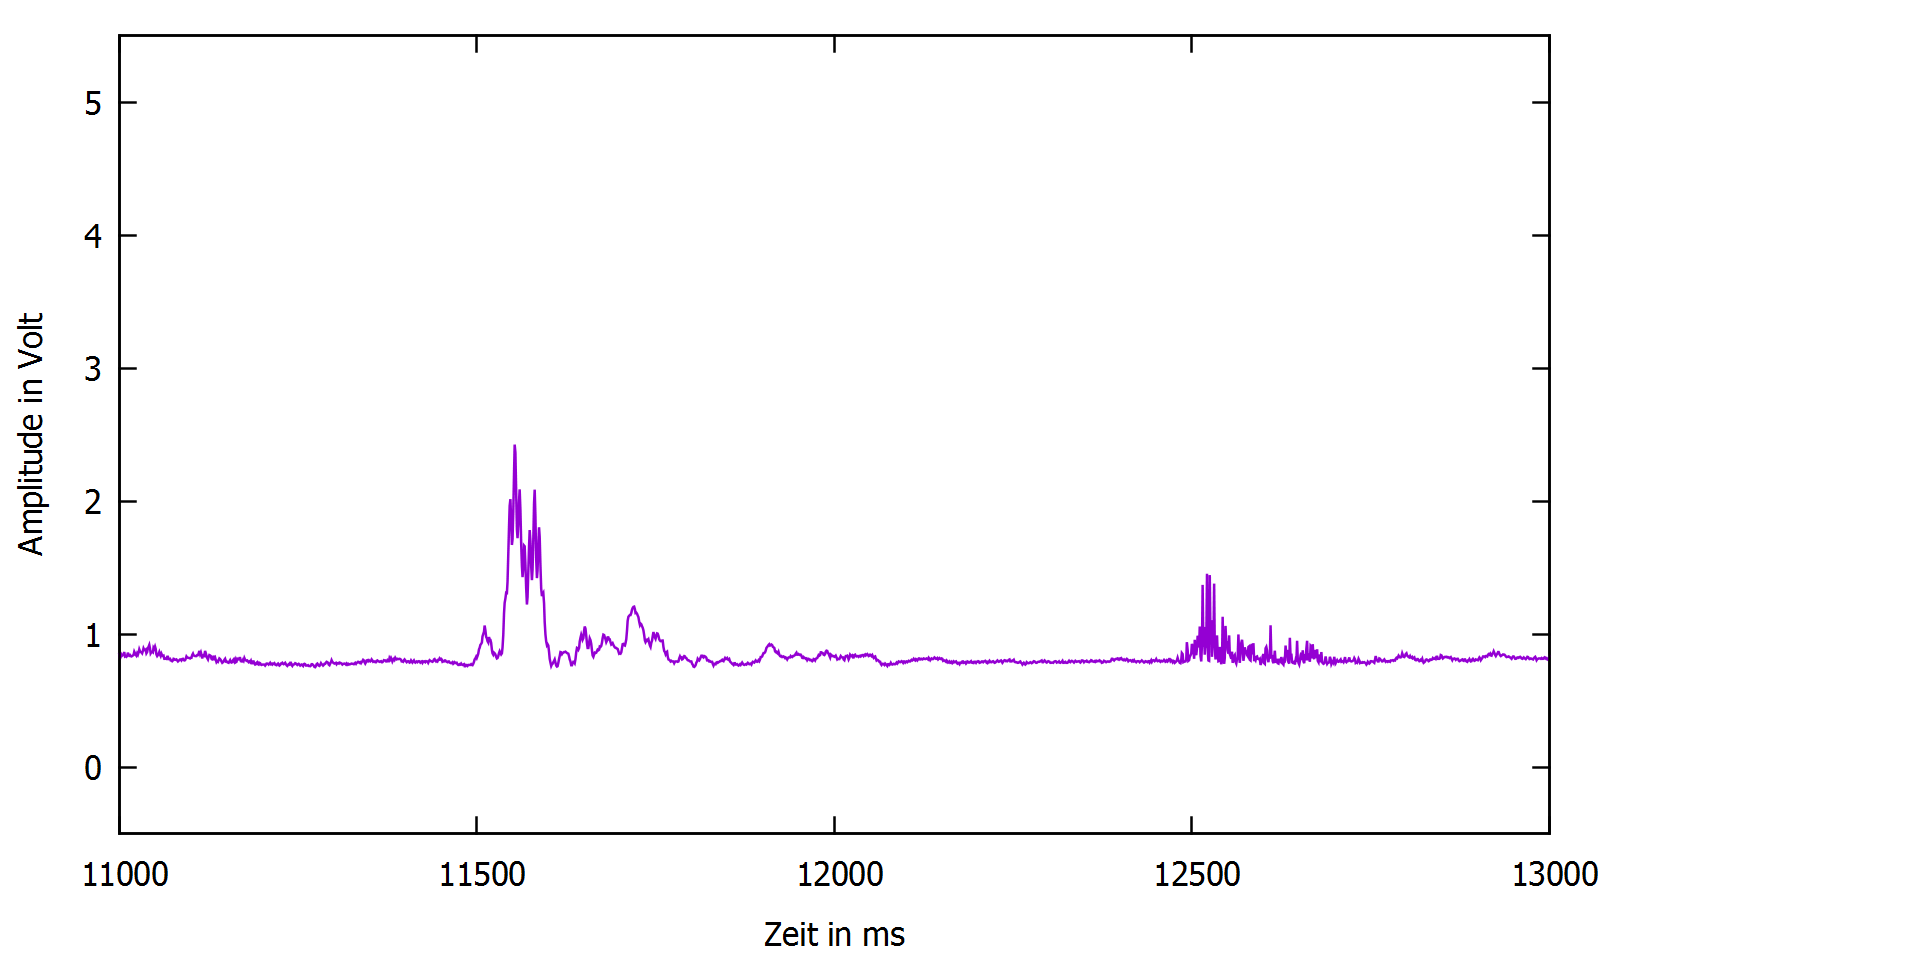
\includegraphics[width=\textwidth]{abklingzeit1.png}
			\caption{kleine kurzzeitige Störung des Messaufbaus}
			\label{bea}
		\end{subfigure}
		\begin{subfigure}{0.8\textwidth}
			\centering
			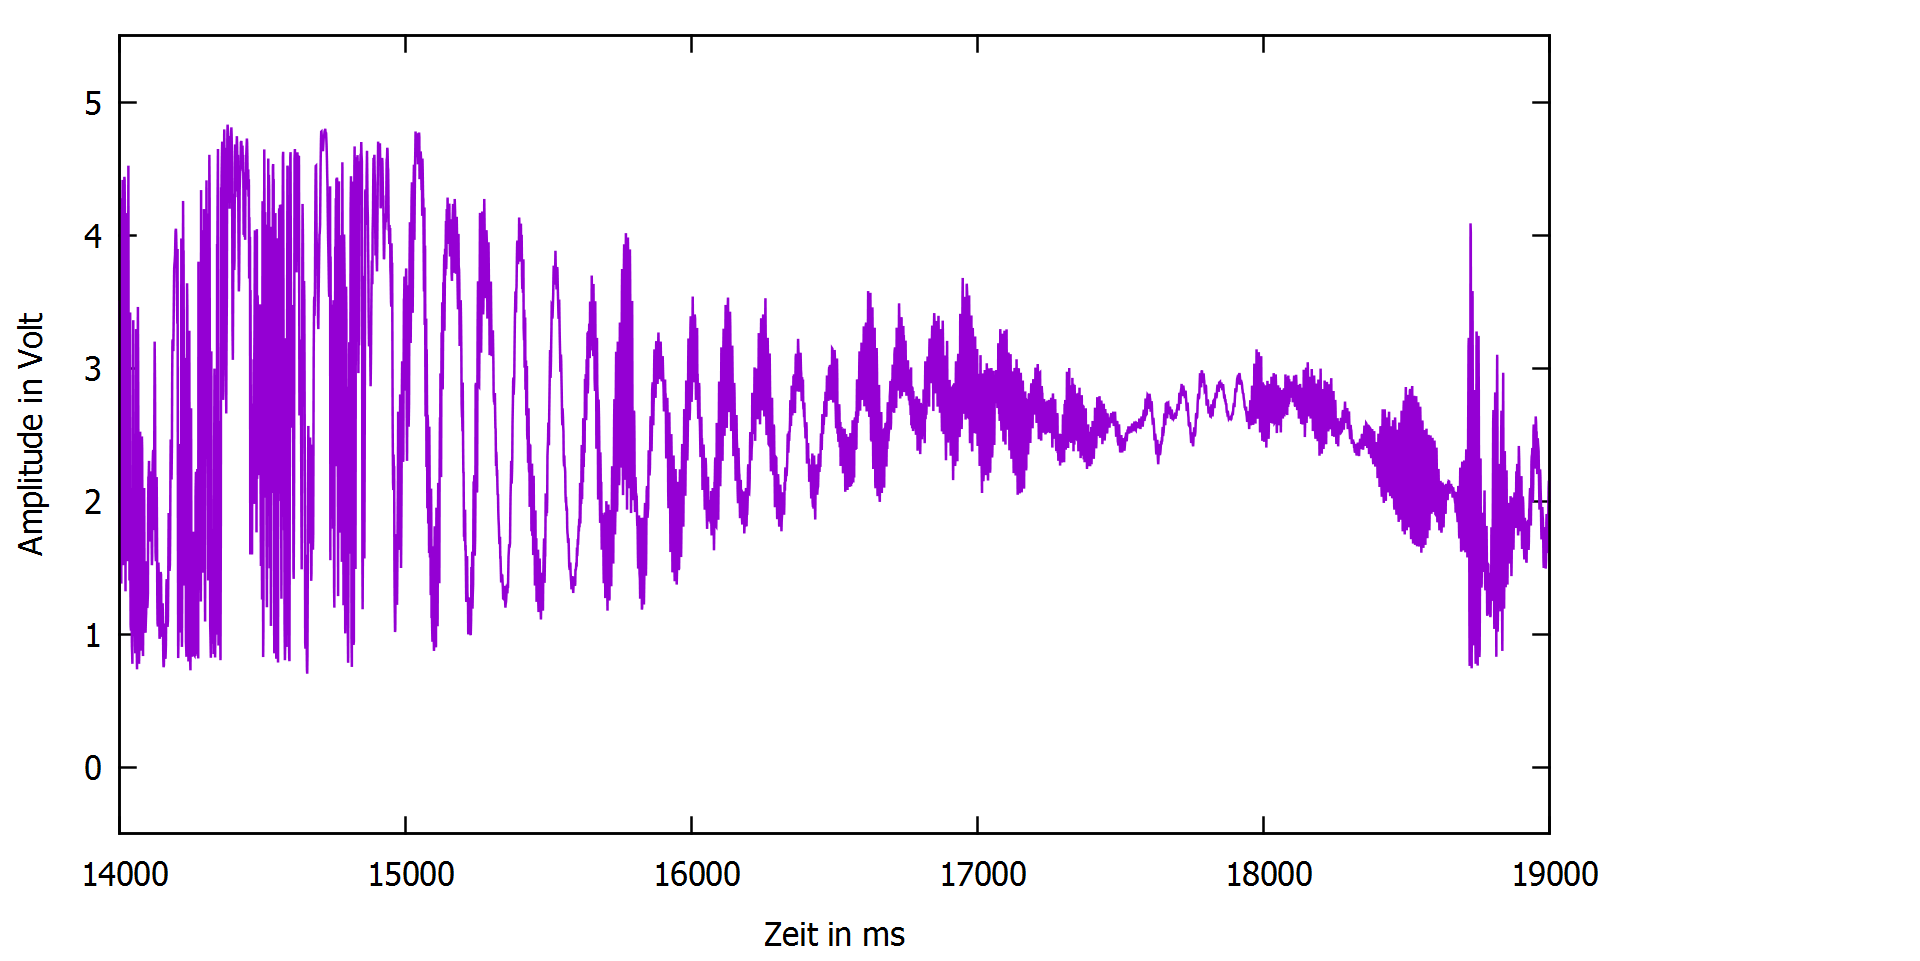
\includegraphics[width=\textwidth]{abklingzeit2.png}
			\caption{Große Störung des Messaufbaus durch Rütteln am Untergrund des Versuchsaufbaus}
			\label{beb}
		\end{subfigure}
		
		\caption{Beruhigung des Messaufbaus nach Störungen}
		\label{be1}
	\end{figure}

\section{Diskussion}

Mithilfe eines Michelson-Interferometers haben wir die Kohärenzlänge des von uns verwendeten He-Ne-Lasers auf $(24,5 \pm 0,6)cm$ bestimmt. Diese Länge stimmt mit den theoretischen Werten überein. He-Ne-Laser haben abhängig von ihrer Resonatorlänge oftmals eine Kohärenzlänge zwischen $20cm$ und $30cm$. Die Kohärenz des Lasers genügt, um Hologramme zu erzeugen, da der dafür benötigte Weglängenunterschied zweier Laserstrahlen aus gleicher Quellen kleiner, als die Kohärenzlänge des He-Ne-Lasers ist.

In einer Störungsmessung konnte gezeigt werden, dass der Versuchsaufbau sehr empfindlich gegenüber Störungen ist. Der Grund dafür ist, dass bereits eine kleine Änderung des Weglängenunterschieds der Laserstrahlen im Größenbereich der Wellenlänge des Laserstrahls das Interferenzmuster signifikant verändert. Dies muss bei der Aufnahme von Hologrammen beachtet werden, da diese zur Erzeugung stabile Interferenzmuster benötigen.
Während der Aufnahme der Hologramme durften wir deshalb zum Beispiel nicht sprechen (ebenso musste der Raum abgedunkelt werden). Die Hologramme sind, wie beschrieben, im Allgemeinen gut gelungen.

\end{document}